Clase: 03/11/2022

\begin{teorema}[de Residuos]
    Sea $f(z)$ una función analítica en el interior y sobre una curva cerrada y simple $\gamma$, excepto en un número finito de discontinuidades aisladas $a,b,c,\cdots$ en el interior de $\gamma$, cuyos residuos son $a_{-1},b_{-1},c_{-1},\cdots$, respectivamente. Entonces, 
    \begin{align*}
        \int_\gamma f = 2\pi i\left[a_{-1}+b_{-1}+c_{-1}+\cdots\right]
    \end{align*}
\end{teorema}

Aplicaciones
\begin{lema}
    Sea $|F(z)|\leq M/R^k$, donde $z=Re^{i\theta},k>0$ y $M$ es una constante. Entonces, 
    $$\lim_{R\to \infty}\int_\gamma e^{imz}F(z)dz = 0,$$
    de $\gamma$ es la curva indicada a continuación y $m\in \mathbb{R}^+$.
    \begin{figure}[H]
        \centering
        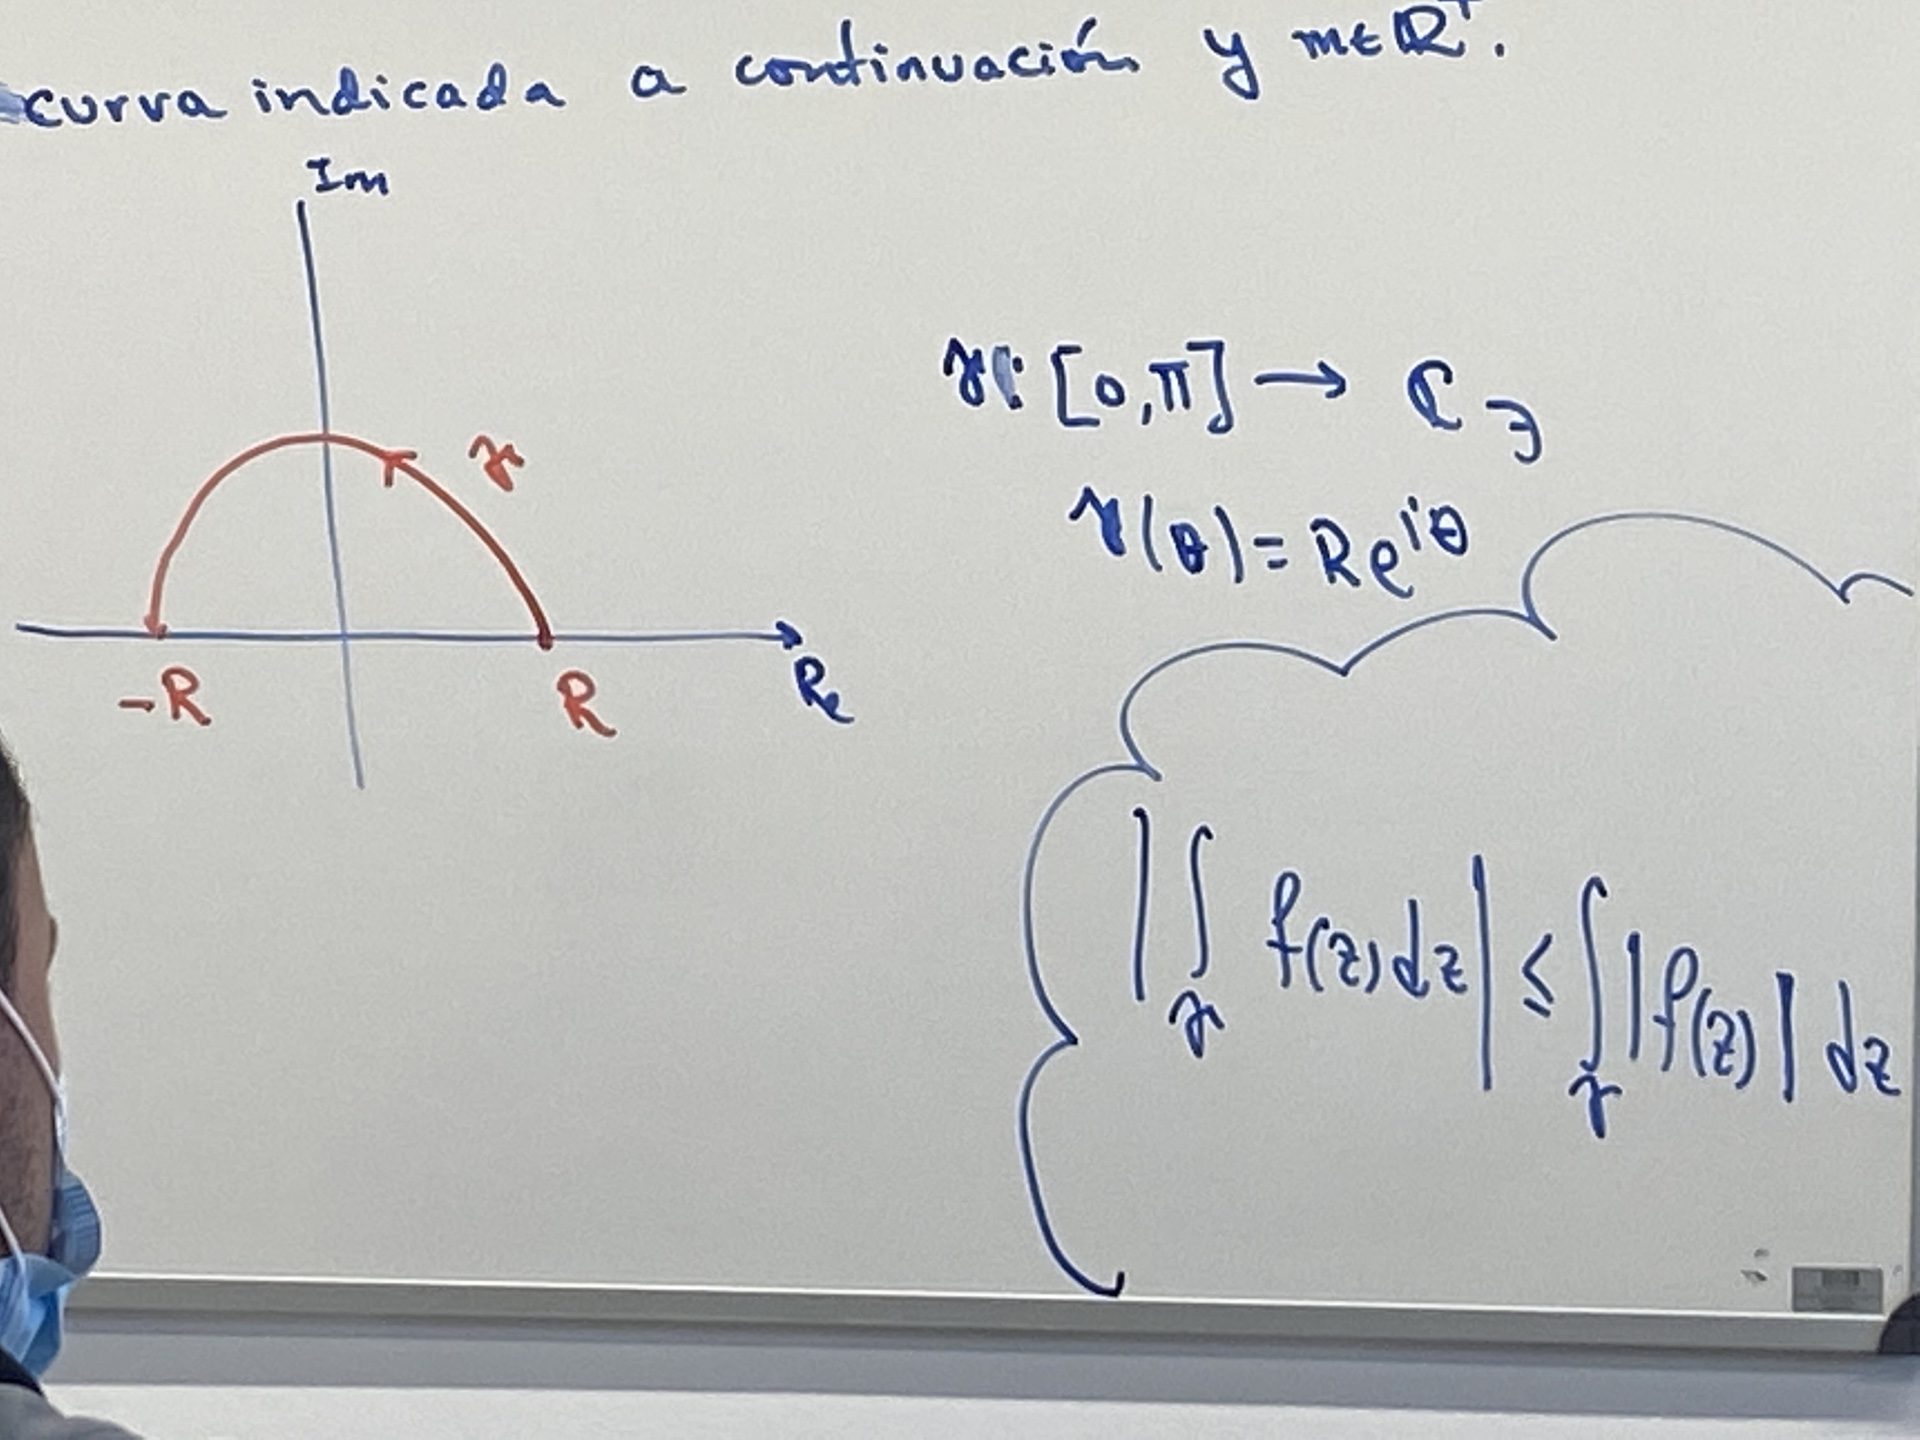
\includegraphics[scale=0.15]{imagenes/25.1}
    \end{figure}
    \begin{figure}[H]
        \centering
        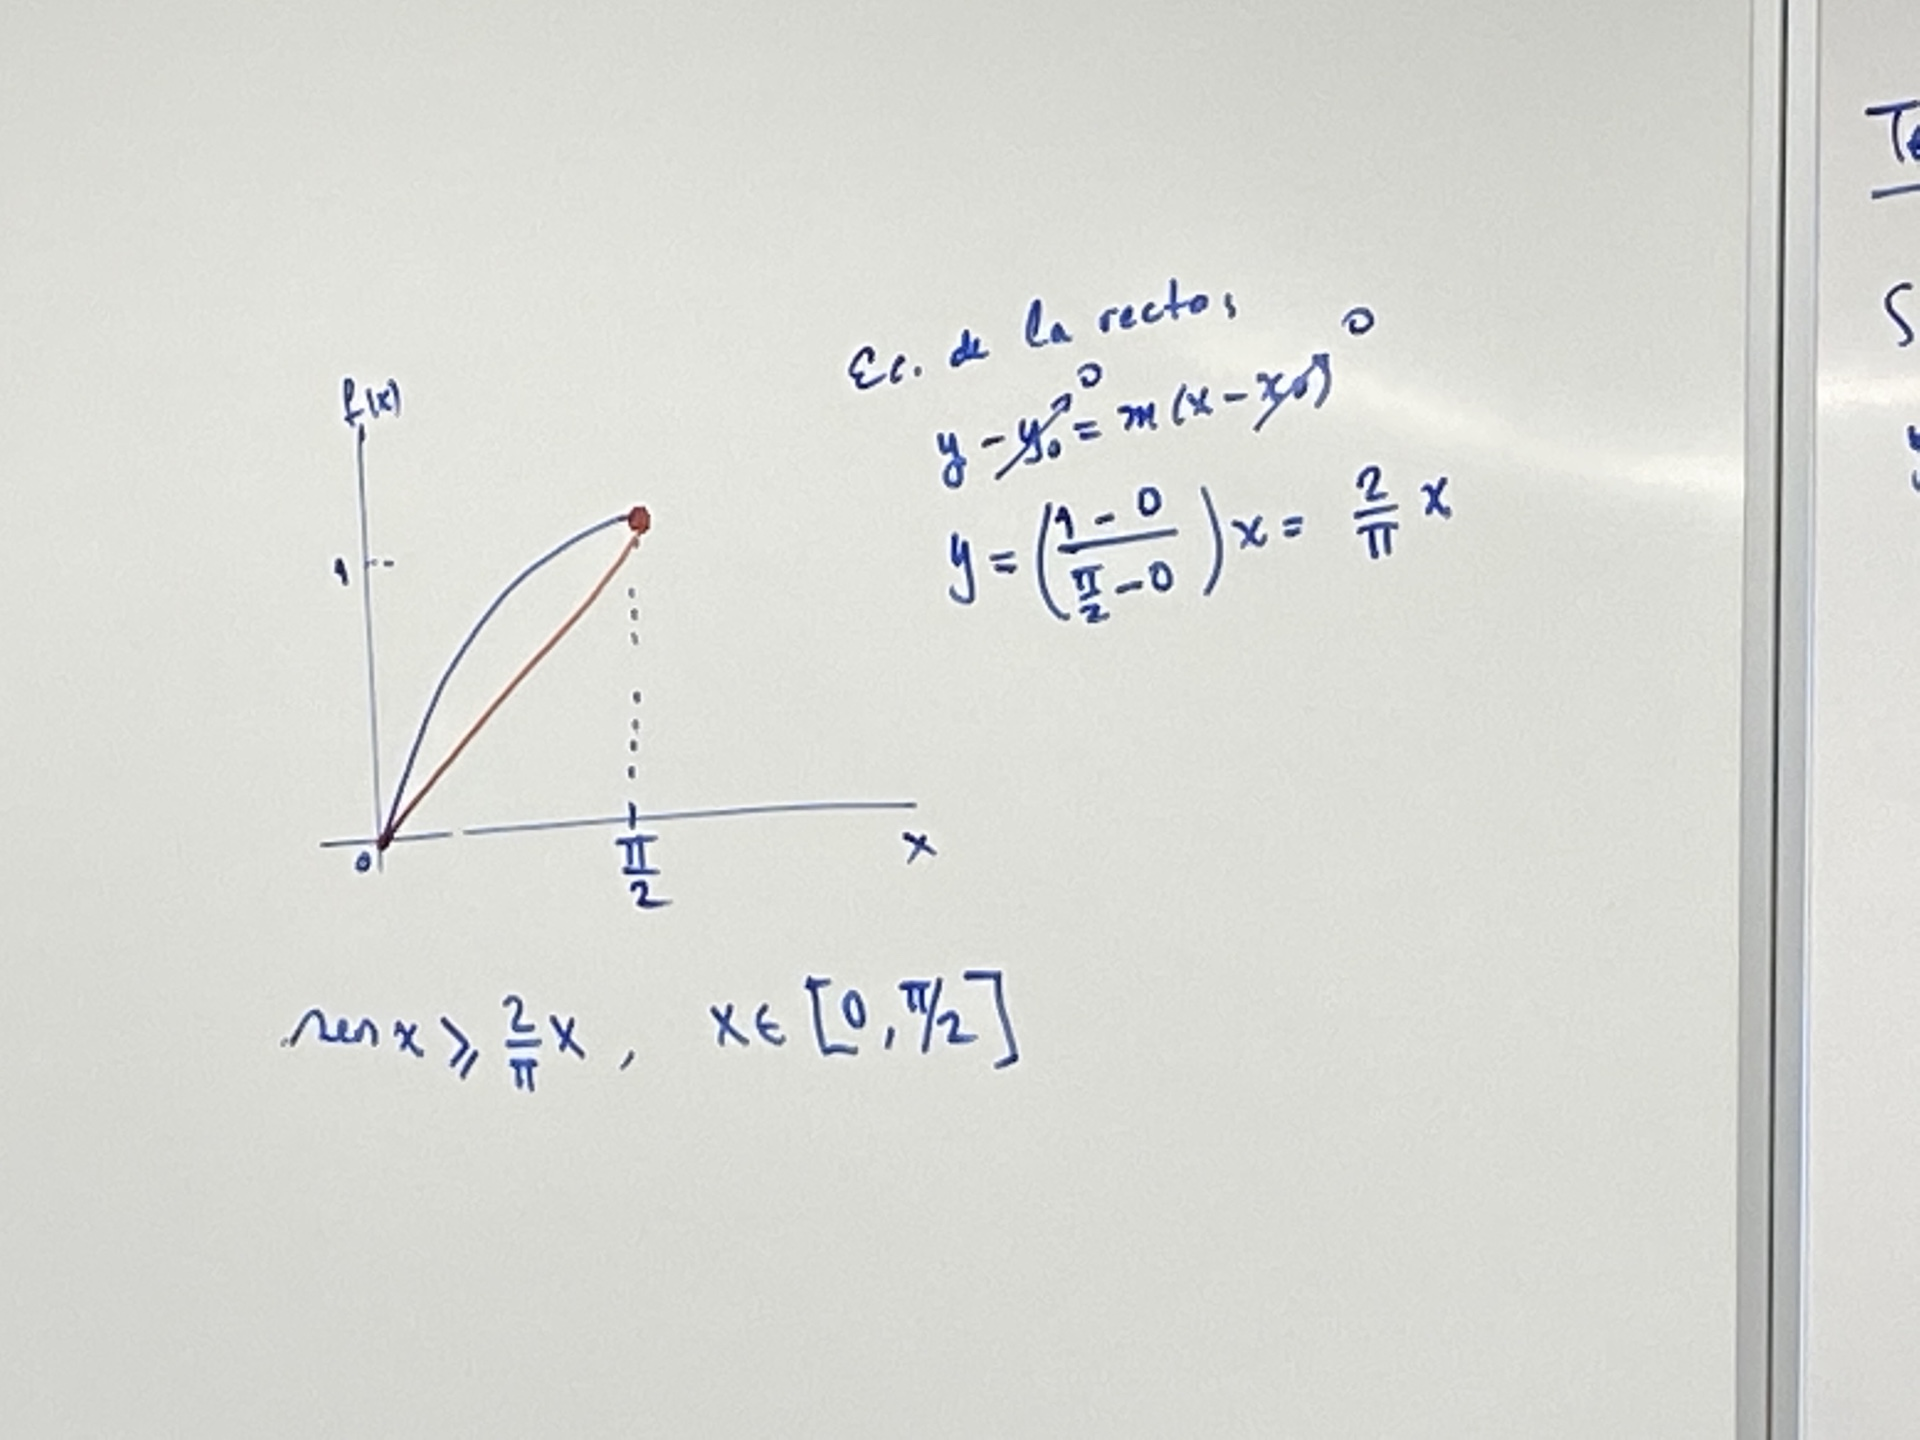
\includegraphics[scale=0.15]{imagenes/25.2}
    \end{figure}
    \begin{dem}
        Sea
        \begin{align*}
            \left|\int_\gamma e^{imz}F(x)dz\right| &= \left| \int_0^{\pi} e^{im Re^{i\theta}}F(Re^{i\theta})\cdot iRe^{i\theta}d\theta \right|\\
            &= \left|\int_0^\pi e^{-mR\sin \theta+imR\cos\theta}\cdot F(Re^{i\theta})\cdot iRe^{i\theta}d\theta\right|\\
            &\leq \int_0^\pi \left| e^{-mR\sin\theta +imR\cos\theta}\right| |F(Re^{i\theta})|\cdot |iRe^{i\theta}|d\theta\\
            &\leq\int_0^\pi e^{-mR\sin \theta}\frac{M}{R^k}\cdot Rd\theta\\
            &= \frac{M}{R^{k-1}}\int_0^{\pi}e^{-mR\sin \theta}d\theta
            \intertext{Nótese que: $\sin\theta\geq 2\theta /\pi, \theta\in[0,\pi/2]$, tal que $e^{-Rm\sin \theta}\leq e^{-Rm(2\theta/\pi)}$. Además, sea $\alpha=\theta/2$ y $2d\alpha = d\theta$}
            &= \frac{M}{R^{k-1}}\int_0^{\pi/2}e^{-mR\sin(2\alpha)}d\alpha\\
            &\leq \frac{2M}{R^{k-1}}\int_0^{\pi/2}e^{-mR\frac{2}{\pi}\left(2\alpha\right)}d\alpha\\
            &= \frac{2M}{R^{k-1}} \left(\frac{-\pi}{4\pi R}\right) e^{-mR\frac{4}{\pi}\alpha}|_0^{\pi/2}\\
            &= \frac{-M\pi}{R^k (2m)}\left[e^{-2mR}-1\right]\to_{R\to\infty}0
        \end{align*}
    \end{dem}
\end{lema}

\begin{ejemplo}
    Compruebe que 
    $$\int_0^{\infty}\frac{\sin x}{x}dx=\frac{\pi}{2}$$
    \begin{sol}
        Sea 
        \begin{enumerate}
            \item Sea $f(z)=\frac{e^{iz}}{z}=\frac{\cos z}{z}+i\frac{\sin z}{z}$. Si $z=x+iy$, con $y=0$, entonces $f(x)=\frac{\cos x}{x}+i\frac{\sin x}{x}$
            \item Sea la trayectoria: 
            \begin{figure}[H]
                \centering
                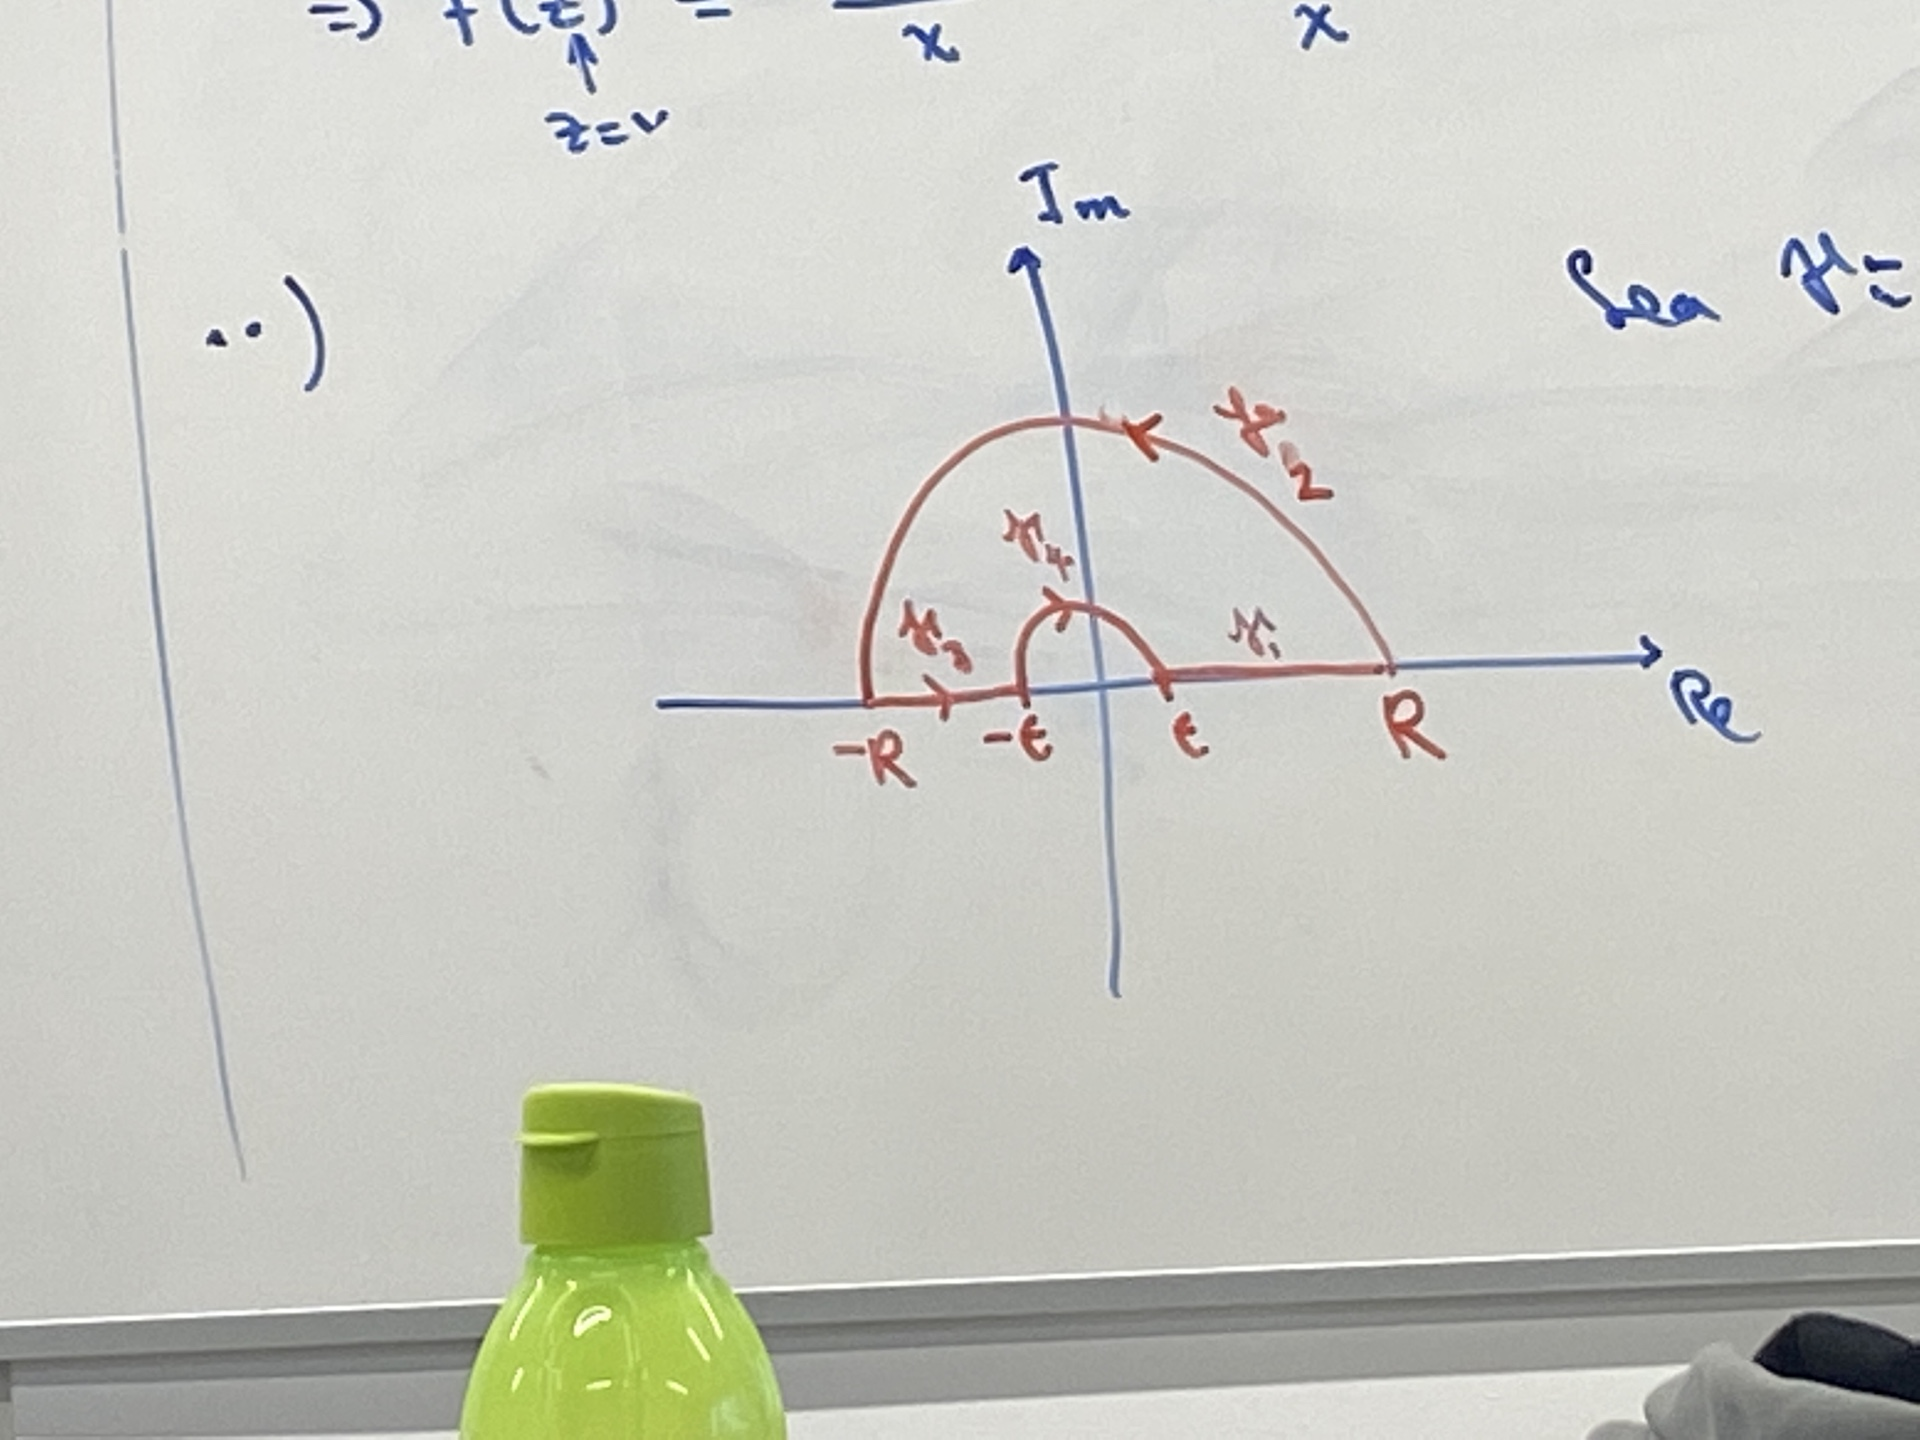
\includegraphics[scale=0.15]{imagenes/25.3}
            \end{figure}
            Sea $\gamma = \gamma_1+\gamma_2+\gamma_3+\gamma_4$, donde
            \begin{align*}
                \gamma_1(t) &= t+0i,\varepsilon \leq t\leq R\\
                \gamma_2(t) &= Re^{it}, 0\leq t\leq \pi\\
                \gamma_3(t) &= t+0i, -R\leq t\leq -\varepsilon\\
                \gamma_4(t) &= \varepsilon e^{it}, \pi \leq t\leq 0
            \end{align*}
            \item Tenemos por teorema de Cauchy
            \begin{align*}
                \int_\gamma f(z)dz &= \int_\gamma \frac{e^{iz}}{z}dz =0
            \end{align*}
            De esto, 
            \begin{align*}
                \int_{\gamma_1}f+\int_{\gamma_2}f+\int_{\gamma_3}f+\int_{\gamma_4}f &= 0\\
                \underbrace{\int_{\varepsilon}^R \frac{e^{it}}{t}}_{A}+ \int_{0}^{\pi} \frac{e^{iRe^{it}}\cdot iRe^{it}}{Re^{it}}dt+\int_{-R}^{-\varepsilon}\frac{e^{it}}{t}df+\int_\pi^0 \frac{e^{i\varepsilon e^{it}}\cdot i\varepsilon e^{it}}{\varepsilon e^{it}} &= 0
            \end{align*}
            Sea 
            \begin{enumerate}
                \item Integral C:
                \begin{align*}
                    \int_{-R}^{-\varepsilon}\frac{e^{it}}{t}dt &=\\
                    \intertext{$t=-\tau$,$dt=-d\tau$}
                    &= \int_{R}^{\varepsilon}\frac{e^{-i\tau}}{-\tau}(-1)d\tau\\
                    &= \frac{R}{\varepsilon} \frac{e^{-i\tau}}{\tau}d\tau = -\frac{\varepsilon}{R}\frac{e^{-i\tau}}{\tau}d\tau\\
                    &= -\int_{\varepsilon}^R\frac{e^{-it}}{t}dt
                \end{align*}
                \item Integral $A+C$: 
                \begin{align*}
                    A+C &= \int_{\varepsilon}^R \frac{e^{it}}{t}dt -\int_{\varepsilon}^R\frac{e^{-it}}{t}dt\\
                    &= \int_{\varepsilon}^R \frac{(e^{it}-e^{-it})}{t}dt\\
                    &= 2i \int_{\varepsilon}^R\frac{\sin t}{t}dt
                \end{align*}
                \item Integral $B$
                \begin{align*}
                    i\int_0^{\pi}e^{iRe^{it}}dt \to_{R\to\infty}0
                \end{align*}
                \item Integral $D$: 
                \begin{align*}
                    i\int_{\pi}^{0} e^{i\varepsilon e^{it}}dt\to_{\varepsilon\to 0}i\int_\pi^0 dt = i\int_{\pi}^0 dt = -i\int_0^{\pi} = -i\pi
                \end{align*}
            \end{enumerate}Entonces, 
            \begin{align*}
                2i\int_0^{\infty}\frac{\sin t}{t}dt &= i\pi
            \end{align*}
        \end{enumerate}
    \end{sol}
\end{ejemplo}